\documentclass[aspectratio=169, 14pt]{beamer}
\usepackage[utf8]{inputenc}
\usepackage{xeCJK}
\usepackage{graphicx}
\usepackage{transparent}
\usepackage[ruled, lined, linesnumbered, commentsnumbered]{algorithm2e}
\usepackage{pgfplots}
\usepackage{tikz}
\usetikzlibrary{matrix,backgrounds}
\usetikzlibrary{arrows}
\usetikzlibrary {arrows.meta}
\usetikzlibrary{calc,shadows.blur,fit,positioning}
\usepackage{minted}
\usepackage{fontawesome5}
\usepackage{booktabs}
\usepackage{caption}
\usepackage{hyperref}
\hypersetup{
    colorlinks=true,
    linkcolor=blue,
    filecolor=magenta,      
    urlcolor=cyan,
    }
\urlstyle{same}
\usetheme{metropolis}
\metroset{block=fill}
\usecolortheme{default}
\definecolor{darkmidnightblue}{rgb}{0.0, 0.2, 0.4}
\definecolor{LightGray}{gray}{0.9}


%------------------------------------------------------------
%This block of code defines the information to appear in the
%Title page
\title[Database Principles and Applications] %optional
{数据库原理与应用}

\subtitle{高级SQL (1)}

\author[CHEN Zhongpu] % (optional)
{CHEN Zhongpu}

\institute[] % (optional)
{
  School of Computing and Artificial Intelligence \\
  \href{mailto:zpchen@swufe.edu.cn}{zpchen@swufe.edu.cn}
}

\date[] % (optional)
{SWUFE, Fall 2022}

%End of title page configuration block
%------------------------------------------------------------


%------------------------------------------------------------
%The next block of commands puts the table of contents at the 
%beginning of each section and highlights the current section:

% \AtBeginSection[]
% {
%   \begin{frame}
%     \frametitle{Table of Contents}
%     \tableofcontents[currentsection]
%   \end{frame}
% }
%------------------------------------------------------------


\begin{document}

%The next statement creates the title page.
\frame{\titlepage}

%---------------------------------------------------------
%This block of code is for the table of contents after
%the title page
% \begin{frame}
% \frametitle{Table of Contents}
% \tableofcontents
% \end{frame}
%--------------------------------------------------------
\begin{frame}
    \frametitle{复习}
    \begin{columns}
        \column{.4\textwidth}
        连接类型 (join types):
        \begin{itemize}
            \item \texttt{inner join}
            \item \texttt{left outer join}
            \item \texttt{right outer join}
            \item \texttt{full outer join}
        \end{itemize}
        \column{.6\textwidth}
        连接条件 (join conditions):
        \begin{itemize}
            \item \texttt{natural join}
            \item \texttt{on <predicate>}
            \item \texttt{using (A1, A2, ..., An)}
        \end{itemize}
    \end{columns}
\end{frame}

\begin{frame}[fragile]
    \frametitle{小测试}
给定关系\texttt{student}和\texttt{takes}:
\begin{enumerate}
    \item 请将下面的SQL语句使用Join重写。
    \begin{minted}[bgcolor=LightGray, baselinestretch=1]{sql}
SELECT name, course_id
FROM student, takes
WHERE student.ID = takes.ID;
    \end{minted}
    \item 找到所有未选课的学生的学号。
\end{enumerate}


\end{frame}

{
    % \usebackgroundtemplate{\transparent{0.3}{\begin{picture}
    %     
\includegraphics[height=0.7\paperheight]{cover}
    % \end{picture}    
    % }}
\usebackgroundtemplate{
  \tikz[overlay,remember picture] 
  \node[opacity=0.3, at=(current page.south east),anchor=south east, yshift=2cm,xshift=4cm] {
    
\includegraphics[height=0.6\paperheight]{cover}};
}
    \begin{frame}
        \section{\textcolor{darkmidnightblue}{1. 高级数据类型}}
    \end{frame}
}

\begin{frame}
    \frametitle{1.1 回顾}
我们目前学习了基本的数值类型,字符串类型,布尔类型和特殊的\texttt{null}。

\begin{columns}
    \column{.5\textwidth}
    \begin{itemize}
        \item \texttt{int}
        \item \texttt{float(n)}
        \item \texttt{real, double precision}
        \item \texttt{numeric(p, d)}
    \end{itemize}
    \column{.4\textwidth}
    \begin{itemize}
        \item \texttt{char(n)}
        \item \texttt{varchar(n)}
        \item \texttt{text}
    \end{itemize}
\end{columns}

\end{frame}

\begin{frame}
    \frametitle{1.2 日期和时间类型}
SQL中支持三种基本的与日期和时间相关的数据类型:

\begin{itemize}
    \item \alert{\texttt{date}}:日期(4个数字),用于表示\underline{某年某月某日}。
    \item \alert{\texttt{time}}:一天中的时间,用于表示\underline{时分秒};也可以指定秒的小数点位数,\alert{\texttt{time(p)}}。
    \item \alert{\texttt{timestamp}}:\texttt{date}和\texttt{time}的结合。类似的,也有一个变种\alert{\texttt{timestamp(p)}}。
\end{itemize}
\begin{tikzpicture}
    \node[fill=yellow,blur shadow={shadow xshift=-0.5ex},
    text width=26em,anchor=south west,rounded corners]
    {\texttt{time}和\texttt{timestamp}可以进一步指定时区。};
\end{tikzpicture} 

\end{frame}

\begin{frame}
    \frametitle{其他编程语言中的时间}
很多编程语言中的时间实际上都是从1970年1月1日到此刻的毫秒数,但是它们提供的API差异较大:

\begin{itemize}
    \item \faIcon{java} \texttt{java.util.Date},\texttt{java.util.Calendar},\texttt{java.sql.Timestamp},\texttt{java.time.*}
    \item \faIcon{python} \texttt{time},\texttt{datetime}
\end{itemize}

\end{frame}

\begin{frame}[fragile]
    \frametitle{timestamp}

    \begin{minted}[bgcolor=LightGray, baselinestretch=.8]{sql}
CREATE TABLE tem_sensor(
    id serial PRIMARY KEY,
    temperature real,
    time timestamp
);

INSERT INTO tem_sensor(temperature, time)
VALUES(17.2, timestamp '2022-10-10 10:39:41');

INSERT INTO tem_sensor(temperature, time)
VALUES(17.2, timestamp '2021-06-18');
    \end{minted}
\faIcon{question-circle} \texttt{timestamp}秒的默认精度是小数点后几位?
\end{frame}

\begin{frame}[fragile]
    \frametitle{date和time}

\faIcon{question-circle} \texttt{time}秒的默认精度是小数点后几位?
\begin{minted}[bgcolor=LightGray, baselinestretch=1]{sql}
time '13:00:00'
time '01:00:00 PM'
time '08:30'
\end{minted}

\pause
\faIcon{code} 下面的哪些写法合法?
\begin{columns}
    \column{.5\textwidth}
    \begin{itemize}
        \item \texttt{date '2008-08-08'}
        \item \texttt{date '2008-08-8'}
    \end{itemize}
    \column{.5\textwidth}
    \begin{itemize}
        \item \texttt{date '2008-8-8'}
        \item \texttt{date '2008-08'}
    \end{itemize}
\end{columns}

\end{frame}

\begin{frame}[fragile]
    \frametitle{实用的时间相关函数}

    \begin{minted}[bgcolor=LightGray, baselinestretch=1]{sql}
SELECT current_date, current_time, current_timestamp;

SELECT current_time at time zone 'CCT';
SELECT current_time at time zone 'Asia/Shanghai';

SELECT CAST('2008-08-08' AS date);
SELECT date '2008/08/08';
    \end{minted}

\faIcon{question-circle} 查阅资料,如何得到2008年8月8日距今有多少天?距今100天后是哪天?

\end{frame}

\begin{frame}[fragile]
    \frametitle{interval}
SQL还提供\alert{\texttt{interval}}用于表示时间间隔:

\begin{minted}[bgcolor=LightGray, baselinestretch=1]{sql}

SELECT date '2008-08-08' + interval '1-1';

SELECT time '08:30' + interval '2 hours';

SELECT time '08:30' + interval '02:00';
    \end{minted}

参考\href{https://www.postgresql.org/docs/14/datatype-datetime.html}{Date/Time Types}。

\end{frame}

\begin{frame}[fragile]
    \frametitle{\texttt{extract()}函数}
\alert{\texttt{extract()}}函数可以从给定\texttt{timestamp}或\texttt{interval}中抽取某个字段。基本语法是:

\begin{verbatim}
EXTRACT(field FROM source)
\end{verbatim}

\begin{minted}[bgcolor=LightGray, baselinestretch=1]{sql}
-- PG, MySQL, Oracle
SELECT EXTRACT(year FROM timestamp '2008-08-08');

-- SQL Server
SELECT YEAR('2008-08-08');
        \end{minted}
    

\end{frame}

\begin{frame}[fragile]
    \frametitle{1.3 小数精度问题}

    \begin{tikzpicture}
        \node[fill=blue!30,blur shadow={shadow xshift=-0.5ex},
        text width=26em,anchor=south west,rounded corners]
        {由于二进制表示的限制,浮点数很多时候都是不精确的。};
    \end{tikzpicture} 

    \begin{minted}[bgcolor=LightGray, baselinestretch=1]{python}
# Python
f = 0.3 + 0.3 + 0.3
    \end{minted}

\begin{minted}[bgcolor=LightGray, baselinestretch=1]{sql}
CREATE TABLE product(
    id serial PRIMARY KEY,
    name text,
    price float
);
\end{minted}

\end{frame}

\begin{frame}[fragile]
    \begin{tikzpicture}
        \node[fill=yellow,blur shadow={shadow xshift=-0.5ex},
        text width=26em,anchor=south west,rounded corners]
        {对精度有要求的场景(如价格),建议不要使用 \texttt{float(n)}、\texttt{real}或\texttt{double precision}。};
    \end{tikzpicture} 

    \begin{columns}
        \column{.5\textwidth}
        \begin{table}
            \caption*{product}
            \begin{tabular}{lll}
              \toprule
              id & name & price \\
              \midrule
              1 & a & 0.3 \\
              2 & b & 0.3 \\
              3 & c & 0.3 \\
              \bottomrule
            \end{tabular}
        \end{table}
        \column{.4\textwidth}
        \begin{minted}[bgcolor=LightGray, baselinestretch=1]{sql}
SELECT SUM(price) 
FROM product;
        \end{minted}
    \end{columns}
    
\faIcon{code} 请使用\texttt{ALTER TABLE}将\texttt{name}的类型更改为\texttt{numeric(8, 2)};然后再执行上面的查询。
\end{frame}

\begin{frame}
因此,建议使用\texttt{numeric}或者\texttt{decimal}。

\begin{tikzpicture}
    \node[fill=yellow,blur shadow={shadow xshift=-0.5ex},
    text width=26em,anchor=south west,rounded corners]
    {PG中\texttt{numeric}如果不指定参数,那么就使用系统最大的precision和scale;而SQL标准的默认scale时0。};
\end{tikzpicture} 

此外,针对价格这种对精度有要求的数据,也可以使用整数代替小数;或者使用DBMS的扩展,如PG中的\texttt{money}数据类型(The Postgres Wiki suggests to largely avoid it, except for those narrowly defined cases. The advantage over \texttt{numeric} is performance.)。
\end{frame}

\begin{frame}[fragile]
    \frametitle{1.4 serial}
有些场景下希望\texttt{id}能够自增,可以使用\texttt{serial}。(类似的还有\texttt{smallserial}和\texttt{bigserial})。

\begin{minted}[bgcolor=LightGray, baselinestretch=1]{sql}
CREATE TABLE product(
    id serial PRIMARY KEY,
    name text,
    price numeric(8, 2)
);
\end{minted}

\faIcon{search} 查阅资料,MySQL的自增如何表示?

\end{frame}

\begin{frame}[fragile]
    \frametitle{More Types}

相较于标准SQL,PG中的类型更加丰富。比如表示空间中点的\texttt{point}:

\begin{minted}[bgcolor=LightGray, baselinestretch=1]{sql}
CREATE TABLE city(
  name varchar(20) PRIMARY KEY,
  location point
);

INSERT INTO city
VALUES ('Chengdu', '(30.5723, 104.0665)');
\end{minted}

\end{frame}

\begin{frame}[fragile]
    \frametitle{1.5 自定义数据类型}
将价格设计成自定义类型:

\begin{minted}[bgcolor=LightGray, baselinestretch=1]{sql}
CREATE TYPE RMB
AS numeric(8, 2);

CREATE TABLE product(
    id serial PRIMARY KEY,
    price RMB
);
\end{minted}

\end{frame}

\begin{frame}[fragile]
考虑健康码的颜色(红、绿、黄),可以为此设计数据类型:

\begin{minted}[bgcolor=LightGray, baselinestretch=1]{sql}
-- PG独有
CREATE TYPE health
AS ENUM ('red', 'yellow', 'green');

CREATE TABLE citizen(
    id serial PRIMARY KEY,
    status health
);
\end{minted}

\end{frame}

\begin{frame}[fragile]
    \section{\textcolor{darkmidnightblue}{2. 类型转换}}
    \begin{minted}[bgcolor=LightGray, baselinestretch=1]{python}
# Python
s = '3.14'
i = int(s)
    \end{minted}
\end{frame}

\begin{frame}[fragile]
    \frametitle{2.1 标准语法}
基本语法是\alert{\texttt{cast(e as t)}},表示将表达式\texttt{e}转化成类型\texttt{t}。   

\begin{minted}[bgcolor=LightGray, baselinestretch=1]{sql}
SELECT CAST('3' AS int) + 1;

SELECT CAST('2008-08-08' AS date);
SELECT date '2008-08-08';
\end{minted}
\pause
不同DBMS提供了都提供了独有的数据类型转化方法,比如PG中的\alert{::}符号:
\begin{minted}[bgcolor=LightGray, baselinestretch=1]{sql}
SELECT '3.14'::DECIMAL;
\end{minted}

\end{frame}

\begin{frame}[fragile]
    \frametitle{2.2 \texttt{to\_xxx()}方法}
PG中还提供了一系列实用的类型转化方法。比如:

\begin{minted}[bgcolor=LightGray, baselinestretch=1]{sql}
SELECT to_date('08-07 2022', 'MM-DD YYYY');
SELECT to_date('22-08-07', 'YY-MM-DD');

SELECT to_char(42, '00999');
SELECT to_char(123, '00999');
\end{minted}

\end{frame}

\begin{frame}[fragile]
    \section{\textcolor{darkmidnightblue}{3. 授权(authorization)}}

    \begin{itemize}
        \item 今年6月,位于密歇根州特洛伊的美国星旗银行称在去年底发生了一次重大数据泄漏事件,受影响的人数154万。
        \item 今年9月,2K确认用户数据遭泄漏,建议用户修改密码保护账户。
        \item 今年10月19日,威胁情报公司SOCRadar宣称其检测到微软由于配置错误而泄露了大量敏感数据。
    \end{itemize}
\end{frame}

\begin{frame}[fragile]
    \frametitle{3.1 授权}
\begin{exampleblock}{授权}
定义存取权限(privilege)即授权。    
\end{exampleblock}

\begin{columns}
    \column{.4\textwidth}<1->
    \begin{itemize}
        \item 授权读取数据
        \item 授权插入新数据
        \item 授权更新数据
        \item 授权删除数据
    \end{itemize}
    \column{.6\textwidth}<2->
\alert{\texttt{GRANT}} <权限列表>
\alert{\texttt{ON}} <关系或视图名>
\alert{\texttt{TO}} <用户或角色>;

\begin{minted}[bgcolor=LightGray, baselinestretch=1]{sql}
GRANT SELECT 
ON department 
TO lilei;
\end{minted}
\end{columns}

\end{frame}

\begin{frame}[fragile]
    \frametitle{3.2 角色}

PG中统一使用role表示用户(user)和用户组(group)。

试着直接运行上面的授权语句,PG会提示报错信息:

\begin{minted}[bgcolor=LightGray, baselinestretch=1]{sql}
GRANT SELECT 
ON department 
TO lilei;
\end{minted}

\begin{quotation}
    \textcolor{red}{[42704] ERROR: role "lilei" does not exist.}
\end{quotation}

\end{frame}

\begin{frame}
查看PG中的所有角色:

\begin{itemize}
    \item 方法一:在DataGrip中左侧「Server Objects」$\rightarrow$ 「roles」
    \item 方法二:通过命令行
\end{itemize}

Windows启动SQLShell,macOS在终端输入\texttt{pgsql mydb},

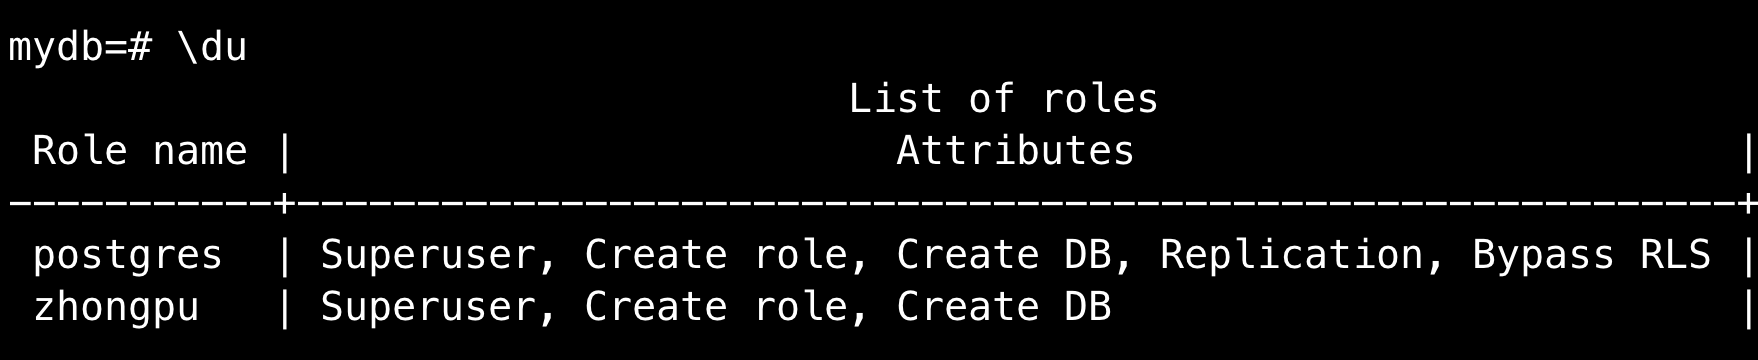
\includegraphics[width=\textwidth]{advanced/du}

\end{frame}

\begin{frame}[fragile]
    \frametitle{创建角色}

    \begin{minted}[bgcolor=LightGray, baselinestretch=1]{sql}
CREATE ROLE hanmeimei;
CREATE ROLE lilei WITH LOGIN PASSWORD '123456';
    \end{minted}
直接\texttt{CREATE ROLE}不具备登录功能;另外注意\texttt{CREATE USER}不是标准语法。

\faIcon{code} 分别使用hanmeimei和lilei连接数据库。
\end{frame}

\begin{frame}[fragile]
    \frametitle{实验}
1. 新角色(lilei)没有权限,所有直接运行下面的查询会报错。
\begin{minted}[bgcolor=LightGray, baselinestretch=1]{sql}
SELECT * FROM department;
\end{minted}
2. 使用postgres角色给lilei授权,然后再运行上面的语句。
\begin{minted}[bgcolor=LightGray, baselinestretch=1]{sql}
GRANT SELECT ON department TO lilei;
\end{minted}
3. 能否直接删除lilei该角色?
\begin{minted}[bgcolor=LightGray, baselinestretch=1]{sql}
DROP ROLE lilei;
\end{minted}

\end{frame}

\begin{frame}
    \frametitle{补充:PG SQL Shell}
PG的SQL Shell提供了若干\href{https://www.postgresql.org/docs/current/app-psql.html}{实用的命令}(不是SQL),比如

\begin{table}
    \begin{tabular}{ll}
      \toprule
      命令 & 含义 \\
      \midrule
      $\backslash$list 或 $\backslash$l & 列出所有数据库 \\
      $\backslash$du & 查看所有角色 \\
      $\backslash$dt & \\
      $\backslash$d <rname> & 查看关系的详情 \\
      $\backslash$conninfo & 查看连接情况 \\ 
      $\backslash$connect <dbname> & 连接数据库 \\
      \bottomrule
    \end{tabular}
\end{table}

\end{frame}

\begin{frame}
    \frametitle{3.3 \texttt{pg\_dump} 练习}

\begin{columns}
    \column{.6\textwidth}
    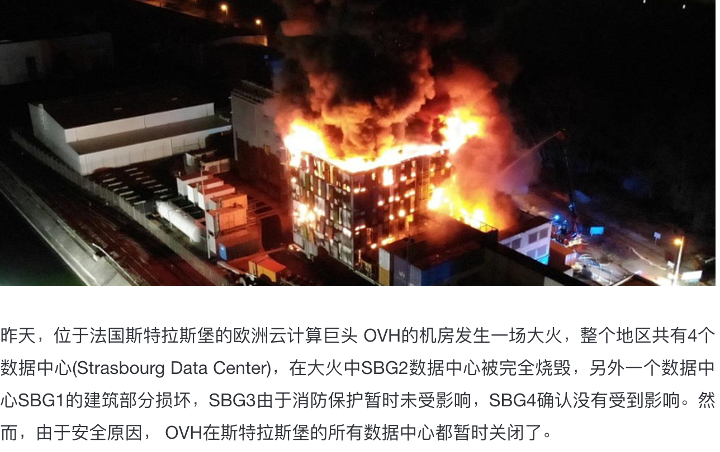
\includegraphics[width=\textwidth]{advanced/fire}
    \column{.4\textwidth}
    数据的备份和恢复对数据安全特别重要。PG中提供了\texttt{pg\_dump}和\texttt{pg\_restore}程序。
\end{columns}

\end{frame}

\begin{frame}

    \begin{columns}
        \column{.6\textwidth}
        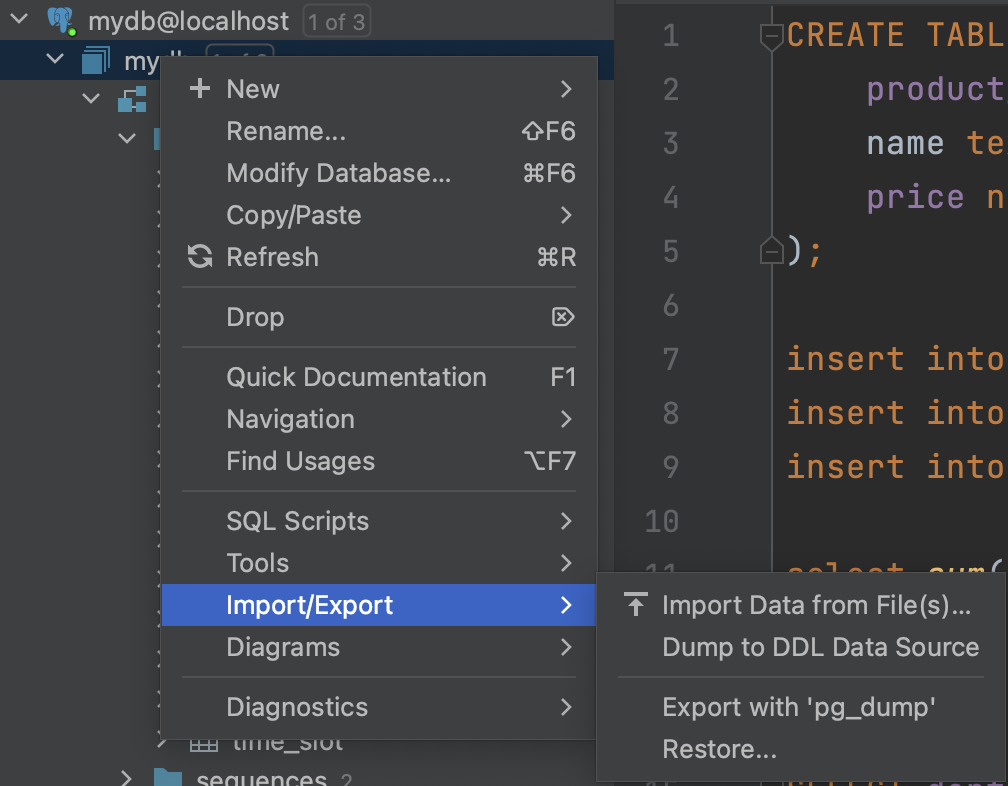
\includegraphics[width=\textwidth]{advanced/dump}
        \column{.4\textwidth}
        \faIcon{code} \textbf{小任务}:完成后查看导出文件的内容。
    \end{columns}
可能需要手动指定\texttt{pg\_dump}程序的位置。macOS上在{\small \texttt{/Applications/Postgres.app/Contents/Versions/latest/bin/pg\_dump}}。
\end{frame}


\begin{frame}[fragile]
    \section{\textcolor{darkmidnightblue}{总结}}

    \begin{itemize}
        \item 高级数据类型(时间和日期)
        \item 类型转化
        \item 授权
    \end{itemize}
\end{frame}

\end{document}